\documentclass{beamer}

\usepackage[utf8]{inputenc}
\usepackage{fancybox}
\usepackage{environ}

\usepackage{tikz}

\beamertemplatenavigationsymbolsempty

\title{1.2 Initial-Value Problems}

\subtitle{a lesson for MATH F302 Differential Equations}

\author{Ed Bueler, Dept.~of Mathematics and Statistics, UAF}

\date{\tiny \today}


\usetheme{Pittsburgh}


\begin{document}

\setbeamertemplate{itemize item}{$\bullet$}
\setbeamertemplate{itemize subitem}{$\circ$}


\begin{frame}
\titlepage

\centerline{\tiny for textbook: \, D. Zill, \emph{A First Course in Differential Equations with Modeling Applications}, 11th ed.}
%\color{green!40!blue}
\end{frame}


\begin{frame}{main purpose of DEs}

\begin{itemize}
\item the main purpose of differential equations (DEs) in science and engineering:

\bigskip

    \centerline{\alert{DEs are models which are capable of prediction}}

\bigskip

\item two things are needed to make a prediction:
\begin{align*}
\begin{matrix}
\text{precise description} \\
\text{of rate of change}
\end{matrix} && \iff && &\text{differential equation} \\
\begin{matrix}
\text{knowledge} \\
\text{of current state}
\end{matrix} && \iff && &\text{initial conditions}
\end{align*}
\item sections 1.1 and 1.2 introduce these two things
\end{itemize}
\end{frame}


\begin{frame}{prediction models}

\begin{itemize}
\item all professionals are skeptics about using math for predictions
\item DEs do \emph{not} ``know the future''
\item \dots but they are \emph{models} which are \emph{capable} of prediction
\item next two slides are examples
\end{itemize}

\bigskip
\begin{quote}
\alert{caution:}  do \alert{not} worry about understanding the specific equations on the next two slides
\end{quote}
\end{frame}


\begin{frame}{an amazingly-accurate \\ real prediction model}

\begin{columns}
\begin{column}{0.55\textwidth}
\begin{itemize}
\item Newton's theory of gravitation gives remarkably-accurate predictions of planets, satellites, and space probes
\item the DEs at right are Newton's model of many particles interacting by gravity,
\item \dots a system of coupled, nonlinear, 2nd-order ODEs for the position $\mathbf{r}_i$ of each object with mass $m_i$
\item adding corrections for relativity makes these predictions practically perfect
\end{itemize}
\end{column}
\begin{column}{0.45\textwidth}
$$\frac{d^2 \mathbf{r}_i}{dt^2} = G \sum_{j\ne i} \frac{m_i m_j}{|\mathbf{r}_j - \mathbf{r}_i|^3} (\mathbf{r}_j - \mathbf{r}_i)$$

\medskip

\quad \tiny \href{https://en.wikipedia.org/wiki/Equations_of_motion}{\texttt{en.wikipedia.org/wiki/Equations\_of\_motion}}
\end{column}
\end{columns}
\end{frame}


\begin{frame}{a pretty-good \\ real prediction model}

\begin{columns}
\begin{column}{0.5\textwidth}
\begin{itemize}
\item \emph{weather prediction} uses Euler's fluid model of the atmosphere
\item \dots a system of PDEs; equations at right
\item predictions have been refined by comparing prediction to what actually happened
\item \dots now we get about 6 days of good/helpful predictions
\item \small \dots and \emph{don't worry} \dots this course is about ODEs and \emph{not} systems of PDEs
\end{itemize}
\end{column}
\begin{column}{0.5\textwidth}
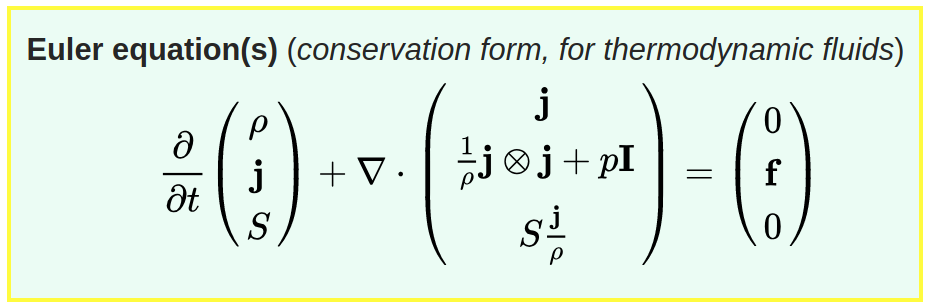
\includegraphics[width=\textwidth]{figs/euler-equations}

\medskip

\quad \tiny \href{https://en.wikipedia.org/wiki/Euler_equations_(fluid_dynamics)}{\texttt{en.wikipedia.org/wiki/}}

\qquad \href{https://en.wikipedia.org/wiki/Euler_equations_(fluid_dynamics)}{\texttt{Euler\_equations\_(fluid\_dynamics)}}
\end{column}
\end{columns}
\end{frame}


\begin{frame}{what kind of student are you?}

\begin{itemize}
\item did you skip the last two slides because you want to know how to do the homework problems quicker?
\item for the students I have taught in math classes I observe that
    \begin{itemize}
    \item better students choose to be curious and interested
    \item better students have at least some tentative trust that teachers are seeking an easy path through the whole subject
    \end{itemize}

\bigskip
\item \dots in any case, there \emph{will} be homework about DE models in section 1.3
\end{itemize}
\end{frame}


\begin{frame}{example 1}

\begin{itemize}
\item \emph{example}: here is the single most important ODE:
    $$y' = y$$
\item it is first-order and linear
\item just by thinking you can write down all of its solutions:
    $$y(x) = \hspace{5.0in}$$
\item and you can graph several particular solutions:

\begin{tikzpicture}[scale=1.0]
  \draw[-latex] (-2,0) -- (2,0) node[xshift=2mm] {$x$};
  \draw[-latex] (0,-1) -- (0,1) node[yshift=2mm] {$y$};
\end{tikzpicture}
\end{itemize}

\vfill
\end{frame}

\begin{frame}{example 1, cont.}

\begin{itemize}
\item but section 1.2 is about initial conditions
\item initial conditions ``pick out'' one prediction (solution) from all the solutions of a differential equation
\end{itemize}

\vfill
\end{frame}

\begin{frame}{example 2}

\begin{itemize}
\item 2nd order
\end{itemize}
\end{frame}

\begin{frame}{general IVP}

\begin{itemize}
\item the general form of an initial-value problem for an ordinary differential equation (ODE IVP) is equation (1) at the start of section 1.2:
\begin{align*}
\frac{d^n y}{dx^n} &= f(x,y,y',\dots,y^{(n-1)}) \\
y(x_0) &= y_0 \\
y'(x_0) &= y_1 \\
   &\vdots \\
y^{(n-1)}(x_0) &= y_{n-1}
\end{align*}
\end{itemize}
\end{frame}

\begin{frame}{Z}

\begin{itemize}
\item X
\end{itemize}
\end{frame}

\begin{frame}{Z}

\begin{itemize}
\item X
\end{itemize}
\end{frame}



\begin{frame}{expectations}

\textbf{expectations}:  to learn this material, just watching this video is \emph{not} enough
\begin{itemize}
\item you need to \emph{read} section 1.2 in the textbook
\item you need to \emph{do} the WebAssign exercises for section 1.2
\item you need to \emph{look around} for other videos and related content; start with the Week 1 page at \href{https://bueler.github.io/math302/}{bueler.github.io/math302}
\end{itemize}
\end{frame}


\end{document}

